\chapter{Simulation Results and Discussion}
\thispagestyle{fancy}

\section{Fractals}
As discussed in section \ref{sec:CAandSOC}, in order to show that a dynamical system exhibits SOC, some fractal nature must be present. As done analytically for a 1-D-model in \cite{fractal_avalanching}, we can plot the energy of a system over time according to the definition of normalized energy
\[
E(t) = \int_f h(x,y,t)^2 df
\]
where $h$ is the height of a site at position $(x,y)$ of the field $f$ at time $t$. In MATLAB/Octave, at the end of every main loop iteration the energy is calculated:
\begin{lstlisting}
ee(t) = sum(sum(f.^2));
\end{lstlisting}
As the energy series in 1-dimensional case shows fractal properties (see \cite{fractal_avalanching}), the question arises if this is true for a 2-dimensional case.

\section{Power-law distributions}

In this section, we investigate tha avalanche size and lifetime distribution, 
according to different boundary conditions, namely the periodic boundary conditions and open boundary conditions.



\section{Power-law distributions}

In this section, we investigate tha avalanche size and lifetime distribution, 
according to different boundary conditions, namely the periodic boundary conditions and open boundary conditions.



\subsection{Periodic boundary conditions}

For periodic boundary conditions, there is never grain lost if we do not introduce friction. 
This means that, in order to study them, we need to be careful with lattice size and driving time, 
in order to not have all the sites overcritical, which will logically imply never-ending avalanches.
As we  also need good statistics to judge the distribution, we must use a reasonably large lattice, 
though in theory, the lattice is infinite large which would imply the size should not matter.

We studied a $100\times 100$ lattice with a driving time $T=5000$, and the results are presented in the figure~\ref{sp}, 
where we see quite a nice power-law behaviour for avalanche size, but a worse one for the lifetime. 
We will give it an explanation by the end of the section, after presenting more results. 
Notice that the first point of both plot, correspond, in fact, to the case where no avalanches occur. 
It is included to show that it is more often the system stays subcritical rather than being overcritical. 



\begin{figure} 
\begin{center}
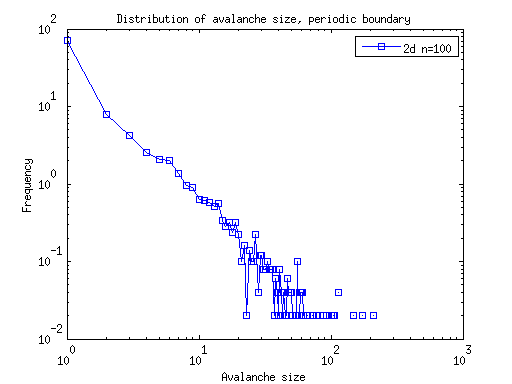
\includegraphics[width=0.49\textwidth]{results/sp.png}
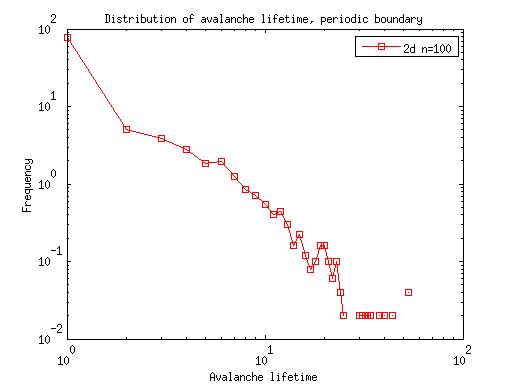
\includegraphics[width=0.49\textwidth]{results/tp.png} 
\caption{Avalanche size and lifetime distribution for $100\times100$ lattice, with periodic boundary conditions. 
The driving time is $T=5000$. }
\label{sp}
\end{center}
\end{figure} 

Due to memory-demanding large lattices and large driving time, we will not treat higher dimensions.
The periodic boundary case without grain lost, though, is not of much interest, as real systems are finite and dissipative.

Instead, we should introduce a friction parameter, and hence, consider a \emph{real} $E$ field, in contrast to a discrete integer field. 
The periodic boundary in principle implies lattice size independence, which will represent a computational advantage, as we can choose small lattice.


We studied this situation for $d=2$, with $n=10$, $n=50$ and $n=100$. See figure~\ref{spf} for the results. 
We see a clear cut-off for large avalanche number due to friction, though the we have a quite nice power-law distribution for small avalanches.
The lifetime is not shown, but it does not differ too much from the case in figure~\ref{sp}.
For the case of $n=100$, we run ten times longer than the other cases, and we see that the distribution for very large avalanches is different from small or medium-size ones. 



Figure~\ref{dsp} shows some plots for higher dimension. The cut-off effect due to friction is much less than the $2d$ lattice, 
but we can increase friction and check again its effect, see figure~\ref{3spf}.
From this analysis, clearly, the dissipation plays an important role, nevertheless, on \emph{average}, 
the total energy of lattice is kept constant when the system evolves, see figure~\ref{ep}. 

Furthermore, for $d=1$, we do not see a power-law distribution, in agreement with the prediction of theory (the situation for open boundary is also checked to be the same). Figure~\ref{1p}. 

\begin{figure} 
\begin{center}
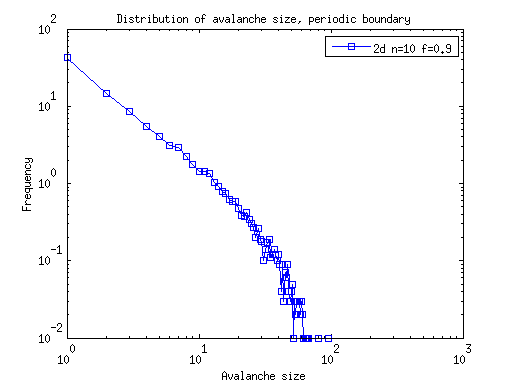
\includegraphics[width=0.49\textwidth]{results/spf.png}
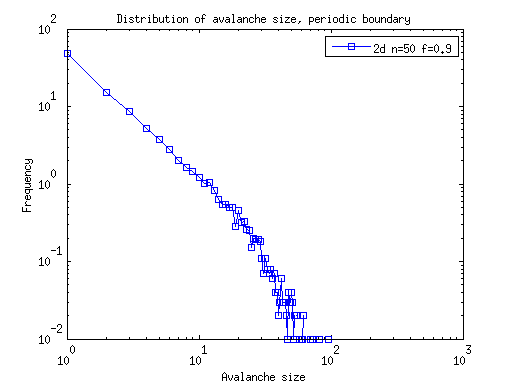
\includegraphics[width=0.49\textwidth]{results/spf50.png} \\
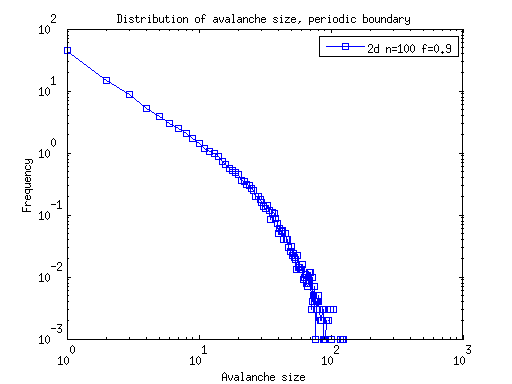
\includegraphics[width=0.49\textwidth]{results/spf100a.png}
\caption{Avalanche size distribution for $2d$ lattice with friction, with periodic boundary conditions. 
The driving time is $T=10000$ for $n=10$ and $n=50$, and $T=100000$ for $n=100$.}
\label{spf}
\end{center}
\end{figure} 



\begin{figure} 
\begin{center}
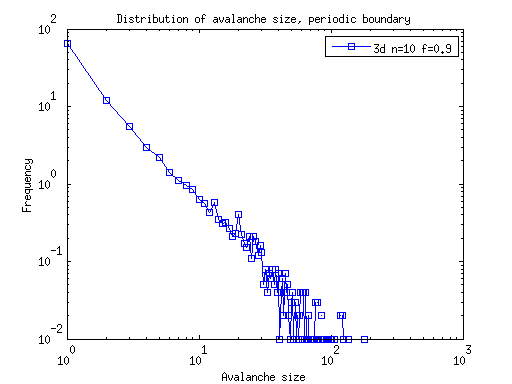
\includegraphics[width=0.49\textwidth]{results/3spf.png}
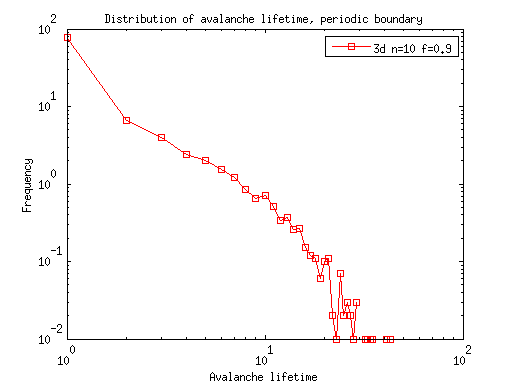
\includegraphics[width=0.49\textwidth]{results/3tpf.png} \\
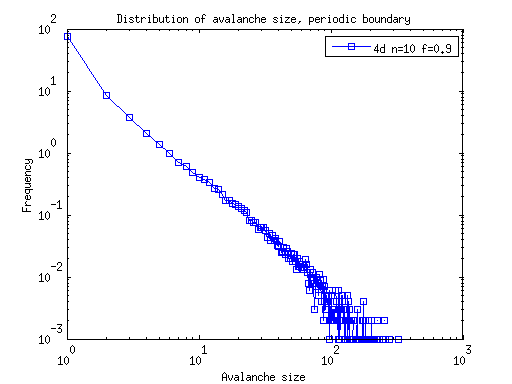
\includegraphics[width=0.49\textwidth]{results/4spf.png}
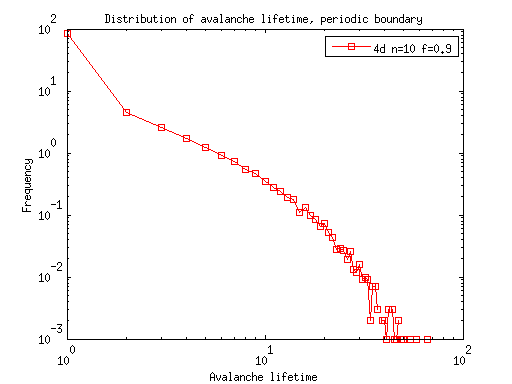
\includegraphics[width=0.49\textwidth]{results/4tpf.png} 
\caption{Avalanche size and lifetime distribution for $3d$ and $4d$ lattices with friction and periodic boundary conditions. }
\label{dspf}
\end{center}
\end{figure}  


\begin{figure} 
\begin{center}
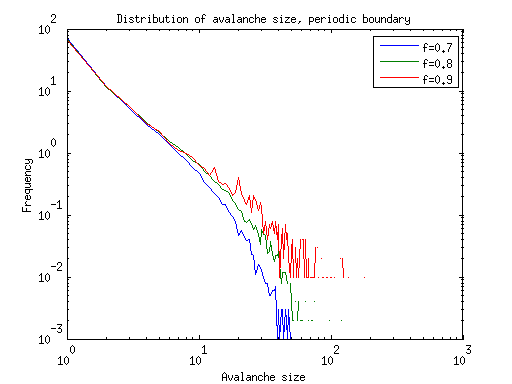
\includegraphics[width=0.49\textwidth]{results/3spfmulti.png}
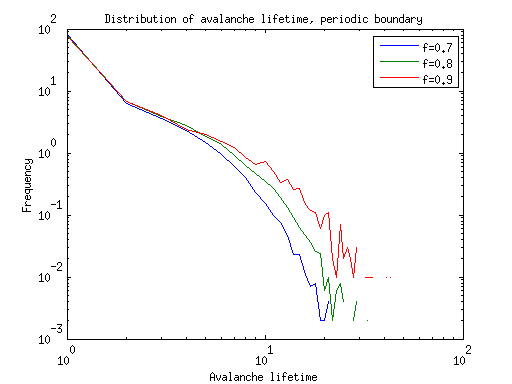
\includegraphics[width=0.49\textwidth]{results/3tpfmulti.png} 
\caption{Avalanche size and lifetime distribution for $3d$ lattice with different friction parameters and periodic boundary conditions. 
The smaller the friction parameter, the larger the dissipation. 
The first point in the lifetime distribution corresponds to zero avalanche during the lifetime.}
\label{3spf}
\end{center}
\end{figure}  

\begin{figure} 
\begin{center}
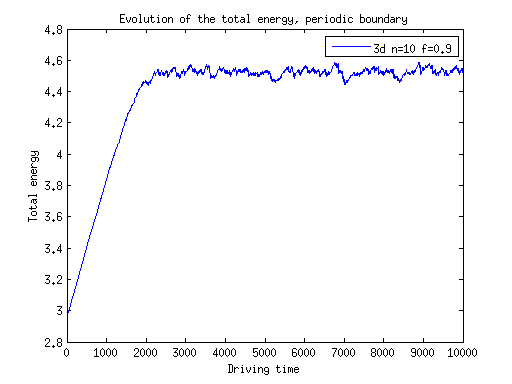
\includegraphics[width=0.49\textwidth]{results/3ep.png}
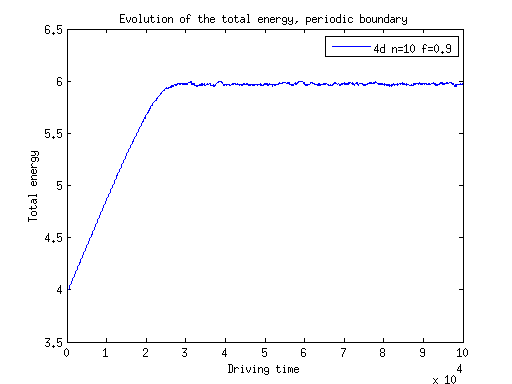
\includegraphics[width=0.49\textwidth]{results/4ep.png} 
\caption{Normalized total energy evolution for $3d$ and $4d$ lattices with friction and periodic boundary conditions. }
\label{ep}
\end{center}
\end{figure}  




\begin{figure} 
\begin{center}
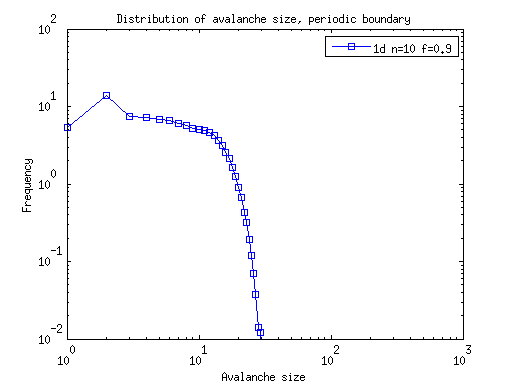
\includegraphics[width=0.49\textwidth]{results/1sp.png}
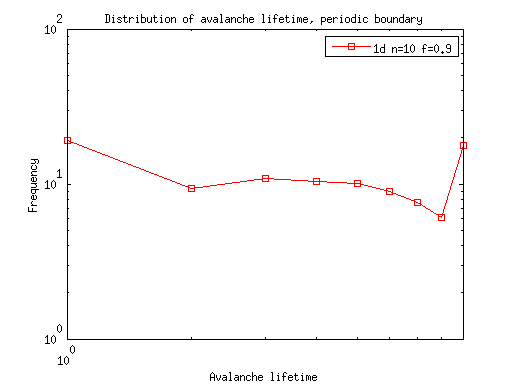
\includegraphics[width=0.49\textwidth]{results/1tp.png} 
\caption{Avalanche size and lifetime distribution for $1d$ lattices with friction and periodic boundary conditions and $T=10^5$. There is no criticality for this case. }
\label{1p}
\end{center}
\end{figure} 








A perturbation in the boundary might give a different avalanche distribution than a perturbation placed in the bulk,
as one might expect that bulk perturbation to produce bigger avalanches, 
because the grain has to be transported further in order to be lost in the boundaries.

We study this effect for 2-dimensional case, and remarkably, we do see different avalanche size distributions (figure~\ref{sv}). 
Furthermore, the high dispersion in large avalanche sizes for the bulk case causes a worse power-law distribution compared to the boundary perturbation case.

For a randomized perturbation sites, the result approaches more to the bulk one. 
\begin{figure} 
\begin{center}
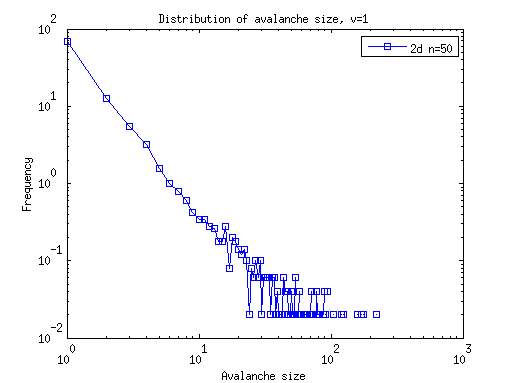
\includegraphics[width=0.49\textwidth]{results/sv1.png}
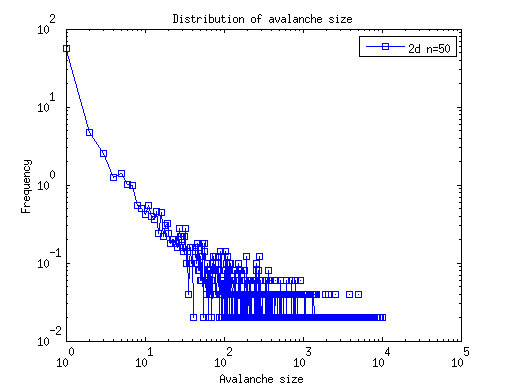
\includegraphics[width=0.49\textwidth]{results/sbulk.png} 
\caption{Avalanche size distribution for $50\times50$ lattice. 
The left one shows the result caused by perturbations in site $(1,1)$, namely in the corner; 
and right one shows the result caused by perturbations in a bulk site, $(25,25)$. The driving time is $T=5000$.  }
\label{sv}
\end{center}
\end{figure} 


The relation of the number of sites in the volume respect to the number of sites at boundary should be proportional to $n$, as it is basically the ration of volume and area.
This implies that for large lattices, one encounters much more large avalanche respect to a smaller lattice. See the plot in the figure~\ref{sn}.

\begin{figure} 
\begin{center}
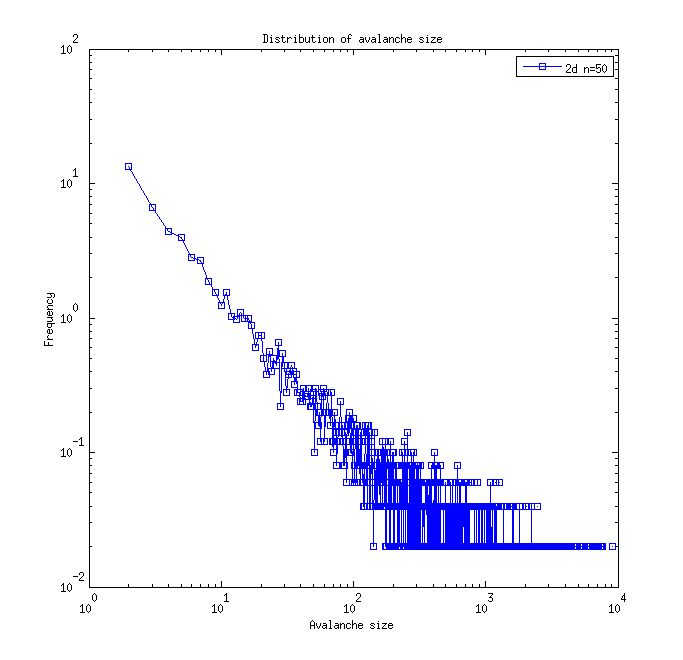
\includegraphics[width=0.49\textwidth]{results/2sn50.png}
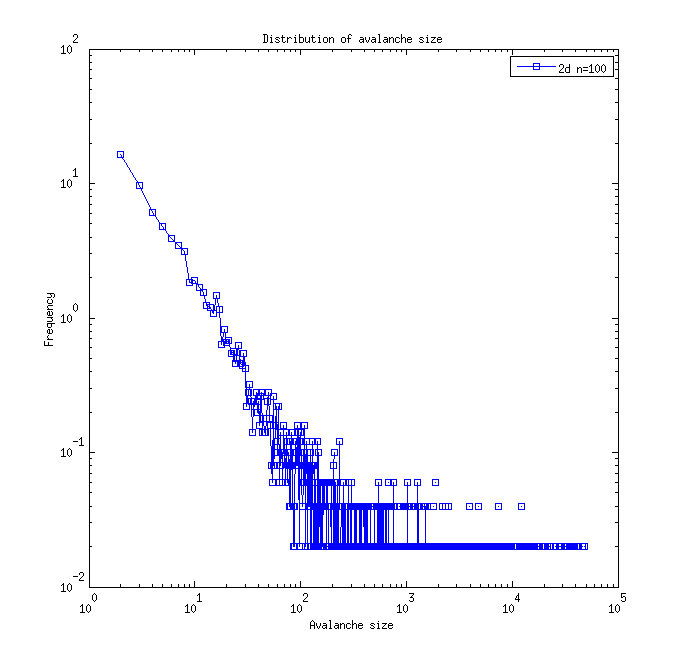
\includegraphics[width=0.49\textwidth]{results/2sn100.png} 
\caption{Avalanche size distribution for $2d$ lattices with different sizes and open boundary conditions.}
\label{sn}
\end{center}
\end{figure} 

If we add friction and go to the real case, the number of huge avalanche reduces. 
Again, we see the importance of friction to modelate the distribution to a more power-law like one, but also with cut-off effect discussed before. 
\begin{figure} 
\begin{center}
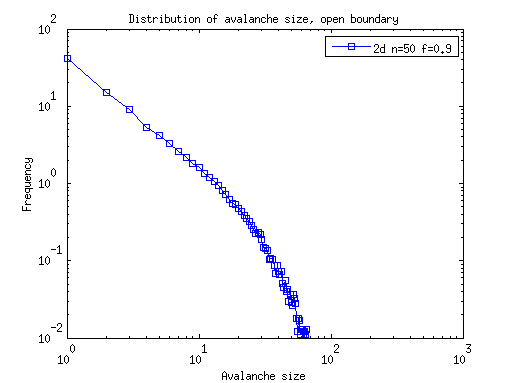
\includegraphics[width=0.49\textwidth]{results/2sof.png}
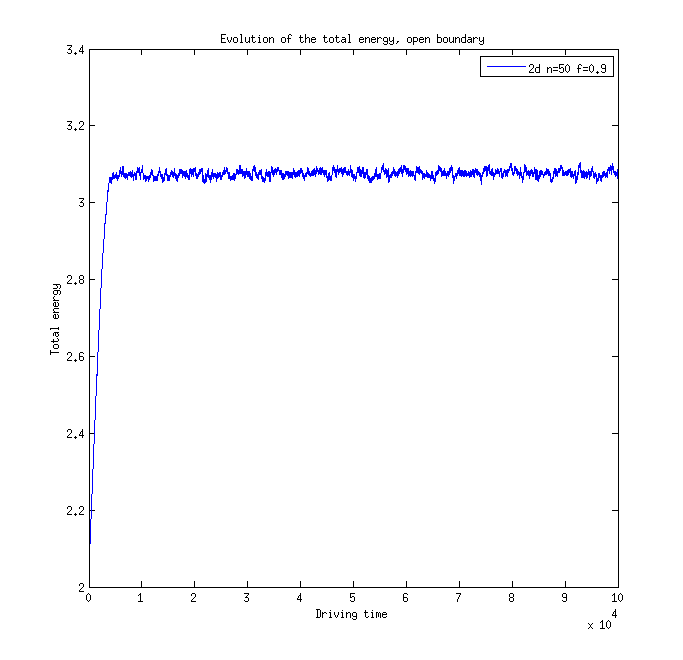
\includegraphics[width=0.49\textwidth]{results/2eof.png}
\caption{Avalanche size distribution and energy evolution for $2d$ lattices with friction and open boundary conditions.}
\label{so}
\end{center}
\end{figure} 




During the driving time, the energy of the system, namely the sum of the values of the field of all sites,
tends to oscillate around a constant value, as the additional grain in each driving time is compensated with the dissipation during avalanche, 
see for example figures~\ref{so} and \ref{ep}.





\subsection{Distribution for small lattices}

Despite we argued that many results, especially avalanche sizes distribution, showed closed to a power-law like distribution, 
except effects of friction or boundary, we here want to understand it, at least qualitatively in a more general way,
to see also why most of avalanche lifetime distribution is not power-law like.


First, let state that the total number of possible configuration states with one site ovecritical is equal to
\[
N_c=n^d\times (2d)^{n^d-1}
\]
where we think of a chain of size $n^d$ (linearize the lattice), and fix one site equal to the critical value 
(i.e. the minimal value that the site will topple, and it is set as $E_c=2d$ for convenience),
but the rest of ($n^d-1$) sites can have a value from $\{0,1, \ldots, 2d-1\}$, so $2d$ values.


However, not all of these configurations will appear during the driving time, as we randomly add only one energy grain to the system for each driving time, 
and the system can dissipate grains, this will soon lead to a characteristic average energy value per site, as we have already seen in some previous plots. 
For example, configurations such that all sites are 0 except of site is overcritical will never occur during the driving time, unless we start with it.
Thus, only a finite subset of it will occur during our simulation. 
The avalanche phenomenon (a set of configuration with one or more than one overcritical states) indeed relates this finite subset with a subset of subcritical configurations.
At contrary, the driving time (the grain adding) do the opposite relation, it makes the system be critical.
This is the mathematical struture behind it, then all the specific rules just change the number of specific site in each subsets,
like 'selecting', and this affects, obviously to the avalanches.

As we have always a discrete lattice in computation, all this relation between the discussed 2 sets exist independently if we run the system or not.
Only that, running the system, we restrict to certain subset, that for our cases, has the total energy per site close to a constant asympototic value.  
This means we just look at certain part of a full complete distribution. 

The avalanches can be characterized by its size (the total number of sites that became overcritical) 
or by its lifetime (the number of different configurations with some sites overcritical). We see that, by definition, 
the values that size can have is bigger than the values of lifetime (as the former refers to number of \emph{sites}, and the latter, to the intermediate \emph{configurations}).
One might expect that lifetime statistics converge faster to the 'exact' distribution. 

To clarify these ideas, let us consider the simplest case of discrete and small lattices with finite boundary.  
The avalanche size and lifetime distribution are shown in the figure~\ref{multi}.
We started with a initial configuration which is \textbf{minimally stable}, i.e., 
all site have a value $E_c-1$, then one grain addition in any of the site will lead to a \emph{catastrophic} avalanche, 
that affects the whole system. 
We might consider these distribution as 'exact' (the subset of 1 state overcritical configurations is almost the whole set, as the system is small enough), 
as running for even larger time, it does not change anymore. 
We can clearly see that these distributions are not power-law like, rather exponetial-like ($y=c^{-x}$). 

What happens for larger lattices is that we are restricting to small and middle large avalanches, so in some sense,
the power-law distribution is an approximation for this regime. 
Catastrophic avalanches that affect to the whole system never happens, except we impose it as initial configuration.
If we start with a zero configuration, this will neither evolve to the minimally stable state (that leads to catastrophic events). 

To check this idea, we run a bigger lattice in 2 dimension, of $50\times 50$ size, with a total driving time $T=10^6$. 
The result of avalanche size distribution is shown in figure~\ref{sfit}, with a respectable power-law fitting over two decades.
The catastrophic avalanches would have a size of order  $10^4$, which occurs for minimally stable states, which will have an average energy per site of
\[
<E>=(n^d(E_c-1)+1)/n^d=E_c-1+1/n^d
\]
which for large lattice, it is $<E>\sim E_c-1$, so $3$ for our case. We can look at the energy evolution that the system evolves to an
average energy per site around $2$ (see figure~\ref{2e}, though it starts with a random initial configuration. 
Starting with a minimally stable state will also converge to the same value).
Hence, we see that many theoretical possible states are strongly supressed. 
A small remnant which is not power-law will stay. One might first consider it as a finite size effect, 
but it is indeed a discrete effect, as we will always have this remnant for any lattice size if we run long enough time, 
due to the system is intrinsically discrete.
Nevertheless, if the system is continuous, which we cannot exactly reproduce with computer simulation, 
then, we have infinite many possible configurations and we can run infinitely large time, 
and should give a power-law distribution, no reason for it to end up abruptly.
Of course, this is our intuition, and it should be proven mathematically, which we will not do this in this project.
Our discussion is only in the qualitative level, that should help to understand better why cellula automata model of sandpile 
generate power-law like distribution.

We saw in some previous plots an accumulated large amount of large events, but also with a lot of dispersion, 
this is mainly statistical fluctuations. Running large enough time, this effect shoul go away and have a distribution like in figure~\ref{sfit}.

Let us now discuss a bit more about the lifetime distribution.  We saw that, quite robustly, it keeps its shape for all the different cases we studied.
The catastrophic avalanches do not have the largest lifetime, and normally, the largest value of lifetime is much less than the total site, unlike avalanche size that can outnumber it.
We show in a table~\ref{tabn2} of catastrophic avalanches in 2 dimensional lattice, and see that the maximum avalanche size is of the order $n^d$, where the lifetime is of the order $n\cdotd$.
Therefore, lifetime should converge faster than avalanche size.

Finally, some last comments on the random set up during the driving time. 
If we always place one grain in the same position in each driving time, 
this will certainly lead to limit cycle, where a finite set of configurations will keep repeating themselves. These states are called recurrent states.
The existence of limit cycles is proven analytically using the abelian property (see Dhar), and we also check it for small lattices, for example
\[ \left( \begin{array}{ccc}
3 & 2 & 2 \\
3 & 4 & 3 \\
0 & 1 & 3 \end{array} \right)\] 
Adding always a grain to the center, a finite configurations repeats. The reader can check it easily by hand or using the \texttt{abelian_sandpile.m} program, 
that can also show the intermediate configurations. This in fact happens to any initial configuration that are attracted to the corresponding limit cycle (they are many different limit cycle depending on where you place the grain).
Furthermore, for periodic boundary condition, with only one grain, the system will infinitely goes into loop between these configurations (maybe this picture corresponds better to the limit cycle notion).
Using randomized grain adding avoids this kind of situation, which are due to discreteness. 





\begin{figure} 
\begin{center}
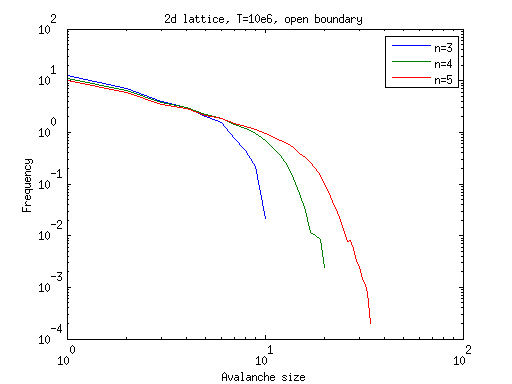
\includegraphics[width=0.49\textwidth]{results/smulti.png}
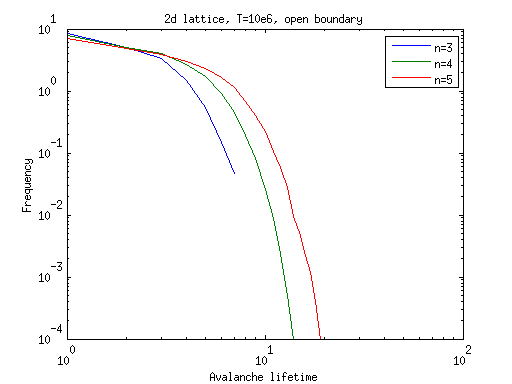
\includegraphics[width=0.49\textwidth]{results/tmulti.png}
\caption{Avalanche size and lifetime distribution for $2d$ small lattices, 
which it started with the all the sites critical. 
These distributions are checked to fit quite well with exponential decaying distributions,
the fitting parameters are not shown, as their value are not meaningful for our discussion.}
\label{multi}
\end{center}
\end{figure} 


\begin{figure} 
\begin{center}
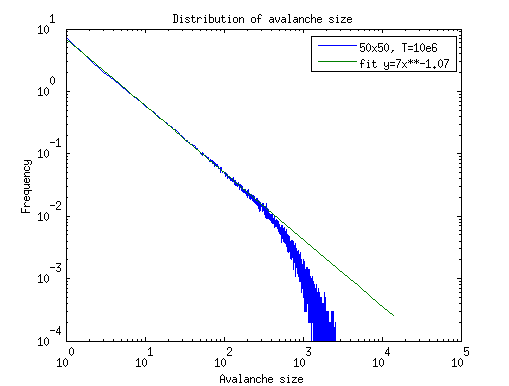
\includegraphics[width=0.49\textwidth]{results/2dsfit.png}
\caption{Avalanche size distribution for $2d$ lattice. }
\label{sfit}
\end{center}
\end{figure} 

\begin{figure} 
\begin{center}
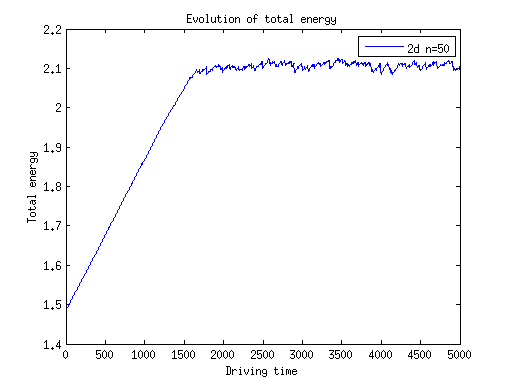
\includegraphics[width=0.49\textwidth]{results/2e.png}
\caption{The evolution of the total energy per site for $2d$ lattice, starting with a random configuration. }
\label{2e}
\end{center}
\end{figure} 

\begin{center}
\begin{tabular}{|c|c|c|c|}
 \hline
 n                  & site  & av. size & av. lifetime\\\hline
 \multirow{3}{*}{3} & (1,1) & 9        & 5 \\ \hline
                    & (1,2) & 9        & 4 \\ \hline
                    & (2,2) & 10       & 3 \\ \hline
 \multirow{3}{*}{4} & (1,1) & 16       & 7 \\ \hline
                    & (1,2) & 16       & 6 \\ \hline
                    & (2,2) & 21       & 5 \\ \hline
 \multirow{6}{*}{5} & (1,1) & 25       & 9 \\ \hline
                    & (1,2) & 25       & 8 \\ \hline
                    & (1,3) & 25       & 7 \\ \hline
                    & (2,2) & 34       & 7 \\ \hline 
                    & (2,3) & 34       & 6 \\ \hline
                    & (3,3) & 35       & 5 \\ \hline
\end{tabular}
\caption{Table with catastrophic avalanches, where the \emph{site} refers to the critical site, while other sites are minimally stable (with value $E_c-1$).}
\label{tabn2}
\end{center} 